\documentclass{scrartcl}

\usepackage{amssymb}
\usepackage{amsmath}
\usepackage{tikz}
\usetikzlibrary{calc,intersections,through,backgrounds,patterns}
\usetikzlibrary{decorations.text, decorations.markings, fit, arrows, arrows.meta}
\usepackage{cancel}

\def\centerarc[#1](#2)(#3:#4:#5)% Syntax: [draw options] (center) (initial angle:final angle:radius)
{ \draw[#1] ($(#2)+({#5*cos(#3)},{#5*sin(#3)})$) arc (#3:#4:#5); }

\begin{document}
	
	%\begin{figure}
	%	\centering
	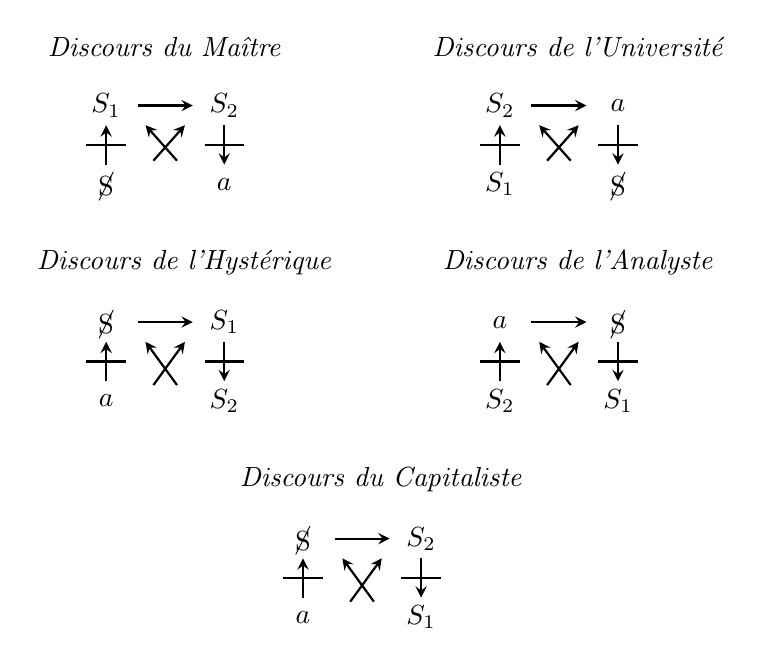
\begin{tikzpicture}
	
	%DISCOURSE OF THE MASTER
	\node at (-0.25,2.75) {\textit{Discours du Ma\^{\i}tre}};
		\node at (-1,2) {$S_1$};
			\draw [thick]	(-1.25,1.5)--(-0.75,1.5);
		\node at (-1,1) {\cancel{S}};
		\node at (0.5,2) {$S_2$};
			\draw [thick]	(0.25,1.5)--(0.75,1.5);
		\node at (0.5,1) {$a$};
	
	%DM arrows
	\draw [->,>=stealth, thick]	(-0.6,2)--(0.1,2);			%horizontal
	\draw [->,>=stealth, thick]	(-1,1.25)--(-1,1.75);		%vertical-up
	\draw [->,>=stealth, thick]	(.5,1.75)--(.5,1.25);		%vertical-down
	\draw [->,>=stealth, thick]	(-0.4,1.3)--(0,1.75);		%diagonal-NE
	\draw [->,>=stealth, thick]	(-0.1,1.3)--(-0.5,1.75);	%diagonal-NW
	
	
	%DISCOURSE OF THE HYSTERIC
	\node at (0,0) {\textit{Discours de l'Hyst\'{e}rique}};
		\node at (-1,-0.75) {\cancel{S}};
			\draw [thick]	(-1.25,-1.25)--(-0.75,-1.25);
		\node at (-1,-1.75) {$a$};
		\node at (0.5,-0.75) {$S_1$};
			\draw [thick]	(0.25,-1.25)--(0.75,-1.25);
		\node at (0.5,-1.75) {$S_2$};
	
	%DH arrows
	\draw [->,>=stealth, thick]	(-0.6,-0.75)--(0.1,-0.75);	%horizontal
	\draw [->,>=stealth, thick]	(-1,-1.5)--(-1,-1);			%vertical-up
	\draw [->,>=stealth, thick]	(.5,-1)--(.5,-1.5);			%vertical-down
	\draw [->,>=stealth, thick]	(-0.4,-1.55)--(0,-1);		%diagonal-NE
	\draw [->,>=stealth, thick]	(-0.1,-1.55)--(-0.5,-1);	%diagonal-NW
	
	
		%DISCOURSE OF THE UNIVERSITY
	\node at (5,2.75) {\textit{Discours de l'Universit\'{e}}};
	\node at (4,2) {$S_2$};
	\draw [thick]	(3.75,1.5)--(4.25,1.5);
	\node at (4,1) {$S_1$};
	\node at (5.5,2) {$a$};
	\draw [thick]	(5.25,1.5)--(5.75,1.5);
	\node at (5.5,1) {\cancel{S}};
	
	%DU arrows
	\draw [->,>=stealth, thick]	(4.4,2)--(5.1,2);			%horizontal
	\draw [->,>=stealth, thick]	(4,1.25)--(4,1.75);			%vertical-up
	\draw [->,>=stealth, thick]	(5.5,1.75)--(5.5,1.25);		%vertical-down
	\draw [->,>=stealth, thick]	(4.6,1.3)--(5,1.75);		%diagonal-NE
	\draw [->,>=stealth, thick]	(4.9,1.3)--(4.5,1.75);		%diagonal-NW
	
	
	%DISCOURSE OF THE ANALYST
	\node at (5,0) {\textit{Discours de l'Analyste}};
		\node at (4,-0.75) {$a$};
			\draw [thick]	(3.75,-1.25)--(4.25,-1.25);
		\node at (4,-1.75) {$S_2$};
		\node at (5.5,-0.75) {\cancel{S}};
			\draw [thick]	(5.25,-1.25)--(5.75,-1.25);
		\node at (5.5,-1.75) {$S_1$};
	
	%DA arrows
	\draw [->,>=stealth, thick]	(4.4,-0.75)--(5.1,-0.75);	%horizontal
	\draw [->,>=stealth, thick]	(4,-1.5)--(4,-1);			%vertical-up
	\draw [->,>=stealth, thick]	(5.5,-1)--(5.5,-1.5);		%vertical-down
	\draw [->,>=stealth, thick]	(4.6,-1.55)--(5,-1);		%diagonal-NE
	\draw [->,>=stealth, thick]	(4.9,-1.55)--(4.5,-1);		%diagonal-NW
	
	
	%DISCOURSE OF THE CAPITALIST
	\node at (2.5,-2.75) {\textit{Discours du Capitaliste}};
		\node at (1.5,-3.5) {\cancel{S}};
			\draw [thick]	(1.25,-4)--(1.75,-4);
		\node at (1.5,-4.5) {$a$};
		\node at (3,-4.5) {$S_1$};
			\draw [thick]	(2.75,-4)--(3.25,-4);
		\node at (3,-3.5) {$S_2$};
		
	%DC arrows
	\draw [->,>=stealth, thick]	(1.9,-3.5)--(2.6,-3.5);		%horizontal
	\draw [->,>=stealth, thick]	(1.5,-4.25)--(1.5,-3.75);	%vertical-up
	\draw [->,>=stealth, thick]	(3,-3.75)--(3,-4.25);		%vertical-down
	\draw [->,>=stealth, thick]	(2.1,-4.3)--(2.5,-3.75);	%diagonal-NE
	\draw [->,>=stealth, thick]	(2.4,-4.3)--(2,-3.75);		%diagonal-NW
		
	\end{tikzpicture}
	%	\caption{...}
	%\end{figure}
	
	\vspace{2cm}
	
	%\begin{figure}
	%	\centering
	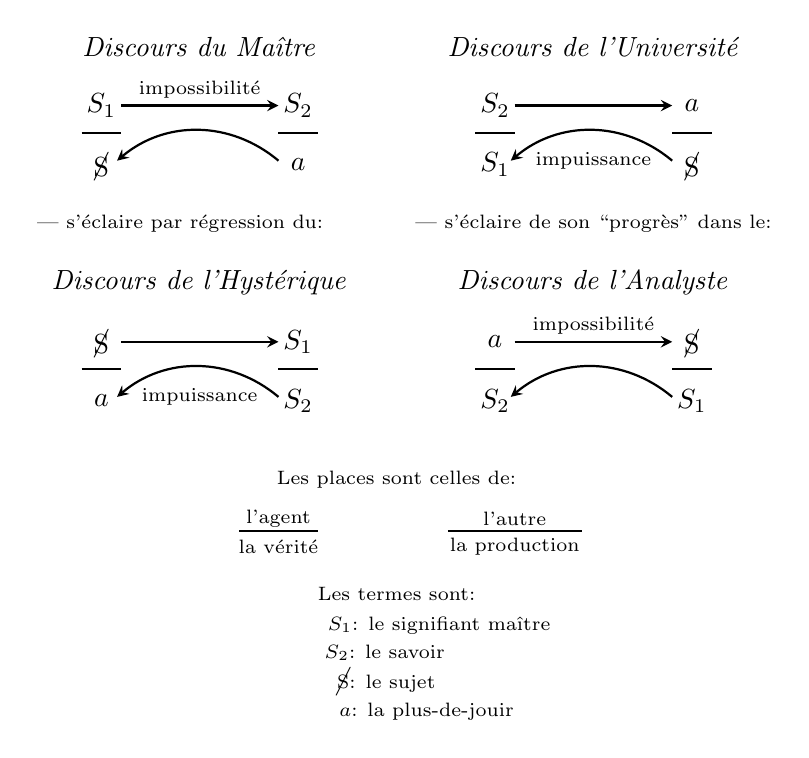
\begin{tikzpicture}
	
	%DISCOURSE OF THE MASTER
	\node at (0,3) {\textit{Discours du Ma\^{\i}tre}};
	\node at (-1.25,2.25) {$S_1$};
	\draw [thick]	(-1.5,1.9)--(-1,1.9);
	\node at (-1.25,1.5) {\cancel{S}};
	\node at (1.25,2.25) {$S_2$};
	\draw [thick]	(1,1.9)--(1.5,1.9);
	\node at (1.25,1.5) {$a$};
	\draw [->,>=stealth, thick]	(-1,2.25)--(1,2.25);	%right arrow
	\node at (0,2.45) {{\scriptsize impossibilit\'{e}}};
	\draw [->,>=stealth, thick]	(1,1.55) to[bend right=40] (-1.05,1.55);
	
	
	\node at (-0.25,0.75) {{\scriptsize | s'\'{e}claire par r\'{e}gression du:}};
	
	
	%DISCOURSE OF THE HYSTERIC
	\node at (0,0) {\textit{Discours de l'Hyst\'{e}rique}};
	\node at (-1.25,-0.75) {\cancel{S}};
		\draw [thick]	(-1.5,-1.1)--(-1,-1.1);
	\node at (-1.25,-1.5) {$a$};
	\node at (1.25,-0.75) {$S_1$};
		\draw [thick]	(1,-1.1)--(1.5,-1.1);
	\node at (1.25,-1.5) {$S_2$};
	\draw [->,>=stealth, thick]	(-1,-0.75)--(1,-0.75);	%right arrow
		\node at (0,-1.45) {{\scriptsize impuissance}};
	\draw [->,>=stealth, thick]	(1,-1.45) to[bend right=40] (-1.05,-1.45);
	
	
	%DISCOURSE OF THE UNIVERSITY
	\node at (5,3) {\textit{Discours de l'Universit\'{e}}};
	\node at (3.75,2.25) {$S_2$};
	\draw [thick]	(3.5,1.9)--(4,1.9);
	\node at (3.75,1.5) {$S_1$};
	\node at (6.25,2.25) {$a$};
	\draw [thick]	(6,1.9)--(6.5,1.9);
	\node at (6.25,1.5) {\cancel{S}};
	\draw [->,>=stealth, thick]	(4,2.25)--(6,2.25);	%right arrow
		\node at (5,1.55) {{\scriptsize impuissance}};
	\draw [->,>=stealth, thick]	(6,1.55) to[bend right=40] (3.95,1.55);
	
	
	\node at (5,0.75) {{\scriptsize | s'\'{e}claire de son ``progr\`{e}s'' dans le:}};
	
	
	%DISCOURSE OF THE ANALYST
	\node at (5,0) {\textit{Discours de l'Analyste}};
	\node at (3.75,-0.75) {$a$};
	\draw [thick]	(3.5,-1.1)--(4,-1.1);
	\node at (3.75,-1.5) {$S_2$};
	\node at (6.25,-0.75) {\cancel{S}};
	\draw [thick]	(6,-1.1)--(6.5,-1.1);
	\node at (6.25,-1.5) {$S_1$};
	\draw [->,>=stealth, thick]	(4,-0.75)--(6,-0.75);	%right arrow
	\node at (5,-0.55) {{\scriptsize impossibilit\'{e}}};
	\draw [->,>=stealth, thick]	(6,-1.45) to[bend right=40] (3.95,-1.45);
	
	
	%LEGEND
	\node at (2.5,-2.5) {{\scriptsize Les places sont celles de:}};
		\node at (1,-3) {{\scriptsize l'agent}};
			\draw [thick]	(0.5,-3.15)--(1.5,-3.15);
		\node at (1,-3.35) {{\scriptsize la v\'{e}rit\'{e}}};
			%
		\node at (4,-3) {{\scriptsize l'autre}};
			\draw [thick]	(3.15,-3.15)--(4.85,-3.15);
		\node at (4,-3.35) {{\scriptsize la production}};
		
	\node at (2.5,-3.95) {{\scriptsize Les termes sont:}};
		\node at (3.04,-4.35) {{\scriptsize $S_1$: le signifiant ma\^{\i}tre}};
		\node at (2.35,-4.7) {{\scriptsize $S_2$: le savoir}};
		\node at (2.37,-5.05) {{\scriptsize \cancel{S}: le sujet}};
		\node at (2.88,-5.45) {{\scriptsize $a$: la plus-de-jouir}};
	
	\end{tikzpicture}
	%	\caption{...}
	%\end{figure}
	
	
	
	\newpage
	
	
	
	%\begin{figure}
	%	\centering
	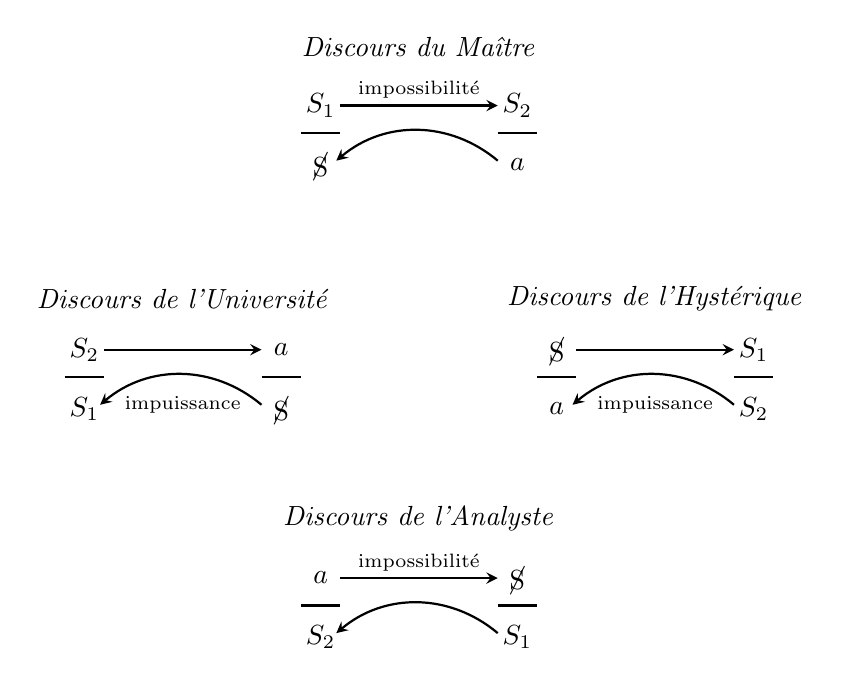
\begin{tikzpicture}
	%DISCOURSE OF THE MASTER
	\node at (0,3) {\textit{Discours du Ma\^{\i}tre}};
	\node at (-1.25,2.25) {$S_1$};
	\draw [thick]	(-1.5,1.9)--(-1,1.9);
	\node at (-1.25,1.5) {\cancel{S}};
	\node at (1.25,2.25) {$S_2$};
	\draw [thick]	(1,1.9)--(1.5,1.9);
	\node at (1.25,1.5) {$a$};
	\draw [->,>=stealth, thick]	(-1,2.25)--(1,2.25);	%right arrow
	\node at (0,2.45) {{\scriptsize impossibilit\'{e}}};
	\draw [->,>=stealth, thick]	(1,1.55) to[bend right=40] (-1.05,1.55);
	
	
	%DISCOURSE OF THE HYSTERIC
	\node at (3,-0.2) {\textit{Discours de l'Hyst\'{e}rique}};
	\node at (1.75,-0.85) {\cancel{S}};
	\draw [thick]	(1.5,-1.2)--(2,-1.2);
	\node at (1.75,-1.6) {$a$};
	\node at (4.25,-0.85) {$S_1$};
	\draw [thick]	(4,-1.2)--(4.5,-1.2);
	\node at (4.25,-1.6) {$S_2$};
	\draw [->,>=stealth, thick]	(2,-0.85)--(4,-0.85);	%right arrow
	\node at (3,-1.55) {{\scriptsize impuissance}};
	\draw [->,>=stealth, thick]	(4,-1.55) to[bend right=40] (1.95,-1.55);
	
	
	%DISCOURSE OF THE UNIVERSITY
	\node at (-3,-0.2) {\textit{Discours de l'Universit\'{e}}};
	\node at (-4.25,-0.85) {$S_2$};
	\draw [thick]	(-4.5,-1.2)--(-4,-1.2);
	\node at (-4.25,-1.6) {$S_1$};
	\node at (-1.75,-0.85) {$a$};
	\draw [thick]	(-2,-1.2)--(-1.5,-1.2);
	\node at (-1.75,-1.6) {\cancel{S}};
	\draw [->,>=stealth, thick]	(-4,-0.85)--(-2,-0.85);	%right arrow
	\node at (-3,-1.55) {{\scriptsize impuissance}};
	\draw [->,>=stealth, thick]	(-2,-1.55) to[bend right=40] (-4.05,-1.55);
	
	
	%DISCOURSE OF THE ANALYST
	\node at (0,-3) {\textit{Discours de l'Analyste}};
	\node at (-1.25,-3.75) {$a$};
	\draw [thick]	(-1.5,-4.1)--(-1,-4.1);
	\node at (-1.25,-4.5) {$S_2$};
	\node at (1.25,-3.75) {\cancel{S}};
	\draw [thick]	(1,-4.1)--(1.5,-4.1);
	\node at (1.25,-4.5) {$S_1$};
	\draw [->,>=stealth, thick]	(-1,-3.75)--(1,-3.75);	%right arrow
	\node at (0,-3.55) {{\scriptsize impossibilit\'{e}}};
	\draw [->,>=stealth, thick]	(1,-4.45) to[bend right=40] (-1.05,-4.45);
	
	%circular arrows
	%\draw[thick,red] (3.35,-1.15) arc (0:360:3.35cm);				%guide for setting the arrows
	\centerarc[->,>=stealth, ultra thick](0,-1.15)(60:25:3.35)		%top-right
	\centerarc[->,>=stealth, ultra thick](0,-1.15)(155:120:3.35)	%top-left
	\centerarc[->,>=stealth, ultra thick](0,-1.15)(345:300:3.35)	%bottom-right
	\centerarc[->,>=stealth, ultra thick](0,-1.15)(240:195:3.35)	%bottom-left
	
	%to make the arrows the same length as the top ones, use:
	%\centerarc[->,>=stealth, ultra thick](0,-1.15)(345:310:3.35)	%bottom-right
	%\centerarc[->,>=stealth, ultra thick](0,-1.15)(230:195:3.35)	%bottom-left
	
	\end{tikzpicture}
	%	\caption{...}
	%\end{figure}	
	
\end{document}